\section{Calculus and Linear Algebra}

\begin{itemize}
    \item logdiff trick can be useful when computing derivatives of functions of the form $f(x)^{g(x)}$.
    \item $\sec$ and $\tan$ work together.
\end{itemize}


\subsection{Limits and derivatives}

\begin{qanda}
    \Q
    What is the derivative of $y = (\log x)^{\log x}$
    \A 
    Taking the natural logarithm of both sides, we have:
    \[
        \log y = \log x \cdot  \log (\log x ).
    \]
    Where we recall that $\frac{d}{dx} \log x = \frac{1}{x}$. Thus, taking derivatives on both sides with respect to $x$ and using the product rule:
    \begin{align*}
        \frac{1}{y} \frac{dy}{dx} 
        &=
        \frac{d}{dx}(\log x) \cdot \log (\log x) + \log x \cdot \frac{d}{dx}(\log (\log x)) \\
        &= \frac{1}{x} \log ( \log x) + \log x \cdot \frac{1}{x} \frac{1}{\log x}.
    \end{align*}

    So:
    \[
        \frac{dy}{dx} = \frac{(\log x)^{\log x}}{x} 
        \left( \log ( \log x) + 1 \right)
    \]
    \emph{This requires some care, I did get some mistakes}
\end{qanda}



\begin{qanda}
    \Q
    Without calculating the numerical results, can you tell me which number is larger: $e^{\pi}$ or $\pi^{e}$?

    \A
    We are interested in determining whether $e^\pi > \pi^e$, which holds if and only if $\pi \log e > e \log \pi$ or $\frac{\log e}{e} > \frac{\log \pi}{\pi}$.
    As such, consider the function $f(x) = \frac{\log x }{x}$, which we want to maximize. The function tends to 0 at $x=0$ and at $x = \infty$, it is continuous and differentiable, so it must have at least a local maximum.
    We can find this:
    \[
        0 = \frac{d}{dx} f(x) = \frac{\frac{1}{x}\cdot x - 1\cdot \log x}{x^2}.
    \]
    For $x \neq 0$, this holds for $1 = ln x$, which implies $x=e$ is the only local (and hence global) maximum.
    This implies $e^pi > \pi^e$.

    \emph{Again, I got it wrong, but reading the first part of the solution helps me remember how to derive the relevant function to maximize}
\end{qanda}

\subsection{Integration}

\begin{qanda}
    \Q
    What is the integral of $\log x$?
    \A
    We proceed with integration by parts:
    \[
        \int 1 \cdot \log x \mathrm{d}x= x \log x - \int x \frac{1}{x} \mathrm{d}x + c = x(\log x - 1) + c.
    \]
\end{qanda}


\begin{qanda}
    \Q
    What is the integral of $\sec(x)$ from $x=0$ to $x=\frac{\pi}{6}$?
    \A
    It is hard to remember the solution from scratch, so we remember to derive relationships of $\sec$ and $\tan$.
    We have:
    \[
        \frac{d \sec(x)}{dx} = \frac{d (\cos x)^{-1}}{dx} = -(-1) \sin x (\cos x)^{-2} = \sec x \tan x \\
    \]
    \[
        \frac{d \tan (x)}{dx} = \frac{d \frac{\sin x}{\cos x}}{dx} = \frac{\cos^2 x - (-\sin^2 x) }{\cos^2 x} = \frac{1}{\cos^2 x} = \sec^2 x.
    \]
    The relationship appears when we consider the sum $g(x) := \sec(x) + \tan(x)$.
    \[
        \frac{d g(x)}{dx} = \sec x (\tan x + \sec x) = \sec x g(x).
    \]
    \emph{What does this mean exactly? Can we step away for one second?}
    We know that:
    \[
        \sec(\pi / 6) - \sec(0) = \int_{0}^{\frac{\pi}{6}} \frac{\mathrm{d}\sec x}{\mathrm{d}x} \mathrm{d}x
    \]
    Here I haven't got an expression in $g(x)$ even though I could add and subtract $\frac{\mathrm{d}\tan x}{\mathrm{d}x}$.
    \emph{So maybe let us go and find $g(x)$}. We know:
    \begin{align*}
        0 &= 
    \frac{\mathrm{d}g(x)}{\mathrm{d}x} - \sec x g(x) \\
          &=
\exp \left( - \int_0^x \sec t \mathrm{d}t \right) \left(  \frac{\mathrm{d}g(x)}{\mathrm{d}x} - \sec x g(x) \right)  \\
          &= \frac{\mathrm{d} \exp \left( - \int_0^x \sec t \mathrm{d}t \right) g(x)}{\mathrm{d}x} 
    \end{align*}
    Integrating both sides yields:
    \[
        c = \exp \left( - \int_0^x \sec t \mathrm{d}t \right) g(x).
    \]
    From which:
    \[
    \int_{0}^{x} \sec t \mathrm{d}t = \log g(x) - \log c.
    \]
    As $\cos(\pi / 6) = \frac{\sqrt{3}}{2}$, we have $\sec(\pi / 6) = \frac{2\sqrt{3}}{3}$ and $\tan(\pi / 6) = \frac{\sqrt{3}}{3}$.
    Thus $g( \pi / 6) = \sqrt{3}$.
    Also, $c = g(0) = 1$. In summary:
    \[
    \int_{0}^{\frac{\pi}{6}} \sec t \mathrm{d}t = \log g(\pi / 6) - 0 = \log \sqrt{3}.
    \]

    \emph{Ok, this is good, but Hugo suggested a faster way to solve this through separation:}
    \[
        I := \int_{0}^{\pi / 6} \sec x \mathrm{d}x =
        \int_{0}^{\pi / 6} \frac{\mathrm{d}g(x)}{\mathrm{d}x} / g(x)\mathrm{d}x 
        .
    \]
    \emph{Substituting $u = g(x)$, we have:}
    \[
    I = \int_{g(0)}^{g(\frac{\pi}{6})} \frac{1}{u} \mathrm{d}u = \ln g(\frac{\pi}{6}) - \ln g(0) = \ln \sqrt{3}.
    \]
\end{qanda}

\begin{qanda} % Applications of integration
    \Q Suppose that two cylinders each with radius 1 intersect at right angles and their centres also intersect. What is the volume of the intersection?

    \A The best thing would be to visualise this. Cross sectionally, from above: 
    
    \begin{figure}[h]
        \centering
        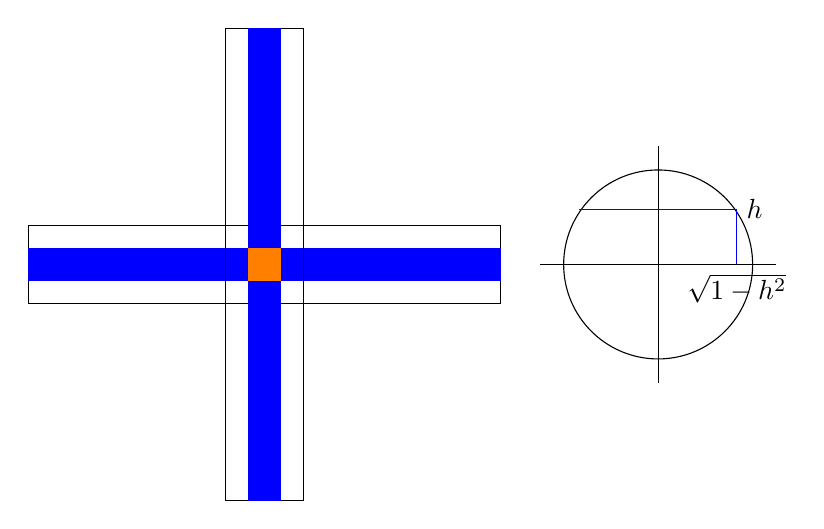
\begin{tikzpicture}
            % center is at 0
            \draw[draw=black] (-3,-.5) rectangle ++(6,1);
            \draw[fill=blue, draw=blue] (-3,-0.2) rectangle ++(6, .4);
            \draw[draw=black] (-.5,-3) rectangle ++(1,6);
            \draw[fill=blue, draw=blue] (-.2,-3) rectangle ++(.4,6);
            \draw[fill=orange, draw=orange] (-0.2,-0.2) rectangle ++(.4,.4);
            \draw[draw=black] (5, 0) circle (1.2);
            \draw[draw=black] (5, -1.5) -- (5, 1.5);
            \draw[draw=black] (3.5, 0) -- (6.5, 0);
            \draw[draw=blue] (4, 0.7) -- (6, 0.7) node[anchor=west] {$h$};
            \draw[draw=blue] (6, 0.7) -- (6, 0) node[anchor=north] { $ \sqrt{1 - h^2}$};
        \end{tikzpicture}
        \caption{In blue: the region of each cylinder which is above $h$. In yellow, the region intersecting both cylinders which is above $h$. }
        \label{fig:}
    \end{figure}

    Without loss of generality, we can focus on the upper-part of the intersection (by symmetry, the top half and the bottom half will have same volume).
    We need to understand the shape of the cross-section at height $h<1$ which is in the intersection of the two cylinders.
    Apparently, this is a square with side $2 \sqrt{1-h^2}$, and so:
    \[
    \frac{V}{2} =
    \int_0^1  4(1 - h^2) \mathrm{d}h = 4 \left(  1 - \frac{1}{3} \right) = \frac{8}{3} 
    \implies
V = \frac{16}{3}.
    \]
\end{qanda}

\begin{qanda} % Snow falling 
    \Q The snow began to fall some time before noon at a constant rate.
    The city of Cambridge sent out a snow plow at noon to clear Massachsusetts Avenue from MIT to Harvard. 
    The plow removed snow at a constant volume per minute.
    At 1 pm, it had moved 2 miles and at 2 pm, 3 miles.
    When did the snow begin to fall?

    \A
    Let us start from scratch.
    Denote by $T<0$ the time at which it started to snow, and let $0$ denote the time at which the plow was started.
    For $t>0>T$, the speed of the plow at time $t$ is inversely proportional to the amount of snow in front of it: $\frac{c_1}{(t-T)}$. The distance travelled up to time $t$ will then be: 
    \[
    D(t):=\int_{0}^{t} \frac{c_1}{u-T} \mathrm{d}u = c_1 (\log(t-T) - \log(-T))
    \]
    We know $D(1) = 2$ and $D(2) = 3$, so we have 2 equations for 2 unknowns:
    \[
        \begin{cases}
            \frac{2}{c_1} = \log \left( \frac{1-T}{-T}  \right) \\
            \frac{3}{c_1} = \log \left( \frac{2-T}{-T}  \right).
        \end{cases}
    \]

    from which:
    \[
    \left( \frac{-T}{1-T} \right)^\frac{1}{2} = \left( \frac{-T}{2-T} \right)^\frac{1}{3} \implies 
    -T (2-T)^2 = (1-T)^3 \implies
    -4T +4T^2 -T^3 = 1 - 3T + 3T^2 - T^3
    \]
    Which simplifies to $T^2 - T - 1 = 0$ with only negative solution: 
    \[
        T_1 = \frac{1 - \sqrt{1 + 4}}{2} = \frac{1 - \sqrt{5}}{2}.
    \]
\end{qanda}

\begin{qanda} % Expected value using integration
    \Q If $X$ is a standard normal random variable $X \sim \text{Normal}(0,1)$, what is $\mathbf{E}[X | X > 0]$?

    \A 
    By definition of expectation:
    \[
        I := \mathbf{E}[X | X > 0] = \int_{0}^{\infty} x \frac{1}{\sqrt{2 \pi}} \exp \left( -\frac{1}{2} x^2 \right) \mathrm{d}x.
    \]
    We substitute $u = x^2 / 2$ so that $\mathrm{d}u = x \mathrm{d}x$:
    \[
    I = \frac{1}{\sqrt{2\pi}} \int_{0}^{\infty}  \exp(-u)\mathrm{d}u = \frac{1}{\sqrt{2 \pi}} .
    \]
    where we can recognize the integral of the exponential pdf.
    In general, for Gaussian random variables $X_\sigma$ with mean 0 and standard deviation $\sigma$, we have 
    \[
        \mathbf{E}[X_\sigma | X_\sigma > 0] =  \sigma E[X_1 | X_1 > 0] = \frac{\sigma}{\sqrt{2\pi}}.
    \]
  
\end{qanda}

\subsection{Partial derivatives and multiple integrals}

\begin{qanda}
    \Q 
    Calculate $I=\int_{0}^{\infty} \exp(-x^2 / 2) \mathrm{d}x$.

    \A
    We can either relate this to the pdf of a standard normal distribution, or alternatively we can use polar coordinates.
    We have: 
    \[
        (2I)^2 = \int_{-\infty}^{\infty} \exp(-x^2 / 2) \, \mathrm{d}x \int_{-\infty}^{\infty} \exp(-y^2 / 2) \, \mathrm{d}y =
\int_{0}^{\infty} \int_{0}^{\infty} \exp(-(x^2+y^2) / 2) \, \mathrm{d}x\mathrm{d}y
    \]
    We use the transformation:
    \[
        \begin{cases}
        x &= r \cos \theta \\
        y &= r \sin \theta
        \end{cases},
    \]
    with $\mathrm{d}x \mathrm{d}y = r \mathrm{d}r \mathrm{d}\theta$.
    As such:
    \[
        (2I)^2 = \int_{0}^{\infty} \int_{0}^{2\pi} \exp \left( -r^2 \right) r  \, \mathrm{d}\theta \, \mathrm{d}r = 2\pi \implies I = \sqrt{\frac{\pi}{2}}.
    \]
\end{qanda}

\subsection{Important Calculus Methods}

These include Taylor Series, Newton's method ($x_{n+1} = x_n - \frac{f(x_n)}{f'(x_n)}$), and the method of Lagrange multipliers.
We also recall the bisection method and the secant method.
In the bisection method we start from an interval whose boundaries are an overestimate and an underestimate of the root. We compute the sign of the function at the midpoint and restart, proceeding by induction.
The secant method is similar to Newton's method, but we approximate the derivative by the slope of the secant line between the last two points.

\begin{qanda}
    \Q
    What is $i^i$?

    \A
    The confusion is that even though we are used to work with imaginary numbers as bases, we can struggle with imaginary exponents.
    However, it is always possible to move the imaginary part to the exponent thanks to Euler's formula. As $i  = \exp \left( i \frac{\pi}{2} \right)$, taking exponents yields:
    \[
     i^i = \exp(-\pi / 2).
    \]
\end{qanda}

\begin{qanda}
  \Q 
  Prove that $(1+x)^n \geq 1 + nx$ for all $x>-1$ and for all integers $n\geq 2$.

  \A
  The simplest way to prove this is through the binomial theorem:
  \[
      (1 + x)^n = \sum_{j=0}^{n} \binom{n}{j} x^j = 1 + nx + x^2\sum_{j=0}^{n-2} \binom{n}{j+2} x^j.
  \]

  We'd need to show that the last sum is non-negative. Not sure exactly how, but induction could work. (obvious for n =2 \ldots)

  Another solution involves Taylor's expansions with intermediate value theorem.
  We consider the function $f(x) = (1 + x)^n$, with first two derivatives equal to: 
  $f'(x) = n (1 + x)^{n-1}$,
  $f''(x) = n(n-1) (1 + x)^{n-2}$.
  For every $x> -1$, there exists $\tilde{x}$ with $|\tilde{x}| \leq x$ such that:
    \[
    f(x) = f(0) + x f'(0) + x^2 \frac{f''(\tilde{x})}{2!} = 1 + nx + x^2 n(n-1)(1+\tilde{x}).
    \]
    All the factors of the last term are non-negative as $n\geq 2$ and $|\tilde{x}| \leq1$, which implies result.
\end{qanda}

\begin{qanda}
    \Q
    Solve $x^2 = 37$ to the third digit.

    \A
    Here, we use Newton's method for the function $f(x) = x^2 - 37$, with $f'(x)=2x$
    We know the solution must be between 6 and 7, and we start with our initial guess $x_0 = 6$.
    Netwon's method proceeds by iterating: $x_{n+1} = x_n - \frac{f(x_n)}{f'(x_n)}$ (analogously as Taylors).
    \[
    x_1 = 6 - \frac{-1}{12} = \frac{71}{12}.
    \]
    The error of this solution is low.
    \[
        \left( 6 + \frac{1}{12} \right)^2 - 37 = 36 + 1 + \frac{1}{144} - 37 = \frac{1}{144} < \frac{1}{100}.
    \]
\end{qanda}


\subsection{Lagrange multipliers}

Let $f\colon \mathbb{R}^n \to \mathbb{R}$ with gradient $\nabla f(x) = \left\langle \frac{\mathrm{d}f}{\mathrm{d}x_1}, \frac{\partial f }{\partial x_2}, \dots \frac{\partial f }{\partial x_n} \right\rangle$.
The necessary condition for maximizing or minimizing $f(x)$ subject to a set of $k$ constraints:
\[
\begin{cases}
  g_1(x_1, x_2, \dots, x_n) = 0, \\
  g_2(x_1, x_2, \dots, x_n) = 0, \\
  \dots \\
  g_k(x_1, x_2, \dots, x_n) = 0,
\end{cases}
\]
is that $\nabla f(x) + \lambda_1 \nabla g_1(x) + \lambda_2 \nabla g_2(x) + \dots + \lambda_k \nabla g_k(x) = 0$, where $\lambda_1, \lambda_2, \dots, \lambda_k$ are called Lagrange multipliers.

\begin{qanda} % Lagrange multipliers example
    \Q What is the distance from the origin to the plane $2x + 3y + 4z = 12$?

    \A 
    The distance from the origin of a point $(x, y,z)$ is $f(x)=\sqrt{x^2 + y^2 + z^2}$.
    There is one constraint $g(x,y,z) = 0$ where $g(x,y,z)=2x + 3y + 4z - 12$.
    At the minimizer, we must have $\nabla f = \lambda \nabla g$, implying:
    \[
        \begin{cases}
            \frac{2x^*}{f(x^*, y^*, z^*)} = 2\lambda, \\
            \frac{2y^*}{f(x^*, y^*, z^*)} = 3\lambda, \\
            \frac{2z^*}{f(x^*, y^*, z^*)} = 4\lambda, \\
            2x^* + 3y^* + 4z^* = 12.
        \end{cases}
        \implies
        \begin{cases}
            3 x^* = 2 y^* \\
            2 x^* = z^* \\
            2x^* + \frac{9}{2}x^* + 8x^* = 12.
        \end{cases}
        \implies 
        \begin{cases}
            x^* = \frac{24}{29} \\
            y^* = \frac{36}{29} \\
            z^* = \frac{48}{29}
        \end{cases}
        ,
    \]
    where the first implication comes from finding expressions of each variable equal to $\lambda f(x^*, y^*, z^*)$.
\end{qanda}

\subsection{Ordinary Differential Equations}

Four ODE pattern commonly seen in interviews:
\begin{itemize}
    \item[\textbf{Separable}] $\frac{dy}{dx} = f(x)g(y)$ which has solution $\int \frac{\mathrm{d}y}{h(y)}\, \mathrm{d}y = \int g(x) \, \mathrm{d}x.$
    \item[\textbf{First-order}] $\frac{\mathrm{d}y}{\mathrm{d}x} + P(x)y = Q(x)$, which are solved through the integrating factor: $I(x) = $
\end{itemize}

\begin{qanda} % Separable ODE 1
    \Q
    Solve the ODE: $y' + 6xy = 0$.

    \A
    This equation is separable as: $\frac{\mathrm{d}y}{\mathrm{d}x} \frac{1}{y} = -6x$. 
    Thus, $\log y = -3 x^2 + c$ and $y \propto  \exp \left( -3 x^2 \right)$.
\end{qanda}

\begin{qanda} % Separable ODE 2
    \Q
    Solve the ODE: $y'= \frac{x-y}{x+y}$.

    \A
    Here the separation is not trivial, because algebra doesn't allow us to find the required form. Instead, we can use change of variables to help us.
    Consider $z=y + x$ so that $z' = y' + 1$. We can rewrite the ODE as:
    \[
    z' - 1 = \frac{2x-z}{z} = \frac{2x}{z} - 1. 
    \implies 
    z'z = 2x
    \implies
    \int  z \, \mathrm{d}z= \int 2x \, \mathrm{d}x  + c
    \]
    \[
     2x^2 + c = z^2 = (x + y)^2 = x^2 + 2xy + y^2 
    \implies 
    x^2 - 2xy - y^2 = c
    \]
\end{qanda}


\subsection{Linear Algebra}

To remember:
\begin{itemize}
    \item \emph{QR decomposition}. For each non-singular $n \times n$ matrix $A$, there is a unique pair of orthogonal matrix $Q$ and upper-triangular matrix $R$ with positive diagonal elements such that $A = QR$
        \footnote{$Q$ corresponds to an orthonormal basis constructed from the original $A$ basis using the Gram-Schmidt process. You can see $R$ as a change of basis, from $Q$ to $A$. Its triangular shape is explained by the fact that vectors from $A$ are incorporated one at a time.}.
\end{itemize}

\begin{qanda}
  \Q 
  There are 3 random variables $X, Y, Z$.
  The correlation between $X$ and $Y$ is 0.8, and 
  the correlation between $X$ and $Z$ is 0.8. 
  What is maximum and minimum correlation between $Y$ and $Z$?

  \A
  The variance covariance matrix is given by:
  \[
      \Sigma = \begin{pmatrix}
    1 & 0.8 & 0.8  \\
    0.8 & 1  & \rho \\
    0.8 & \rho & 1 
  \end{pmatrix}
  \]

  It is obvious that the determinant of the first two leading principals are positive, and so we simply need to find the minimum $\rho$ such that the determinant of the matrix is non-negative.
  The determinant is a quadratic function of $\rho$, and we know $\rho = 1$ is a root. The minimum $\rho$ satisfying the condition is hence the other root. We solve:
  \begin{align*}
      0 &= \text{det}(\Sigma) = (1 - \rho^2) - 0.8^2 (1-\rho) + 0.8^2 (\rho-1) \\
        &= (1-\rho) (1 + \rho - 2 \cdot 0.8^2)
  \end{align*}
  which gives $\rho = 1.28 - 1 = 0.28$ as the smaller root.
\end{qanda}

\begin{qanda}
  \Q
  If the programming language you are using doesn't have a function of the linear least squares regression, how would you design an algorithm to compute it?


  \A
  Given a design matrix $X$, I would compute: 
  \[
      (X^T X)\beta = X^T y \implies \beta = (X^T X)^{-1}  X y.
  \]
  Probably, they want me to use the QR decomposition, so let us write $X^T X = QR$, which means:
  \[
  \beta = R^{-1} Q^T X^T y,
  \]
  where $R^{-1}$ is easy to compute as $R$ is upper triangular. 

  \textcolor{green}{Just treat the equation as
      \[
      Ax = y \implies QRx = y \implies Rx=Q^Ty
      \],
      where the system is easy to solve from \textquote{the bottom up} due to upper-triangularity of $R$.}

\end{qanda}

\subsection{Determinant, eigenvalue and eigenvector}

\begin{qanda} % Eigenvalues and eigenvectors
    \Q What are the eigenvalues and eigenvectors of the matrix $A = \begin{pmatrix}
        2 & 1 \\
        1 & 2
    \end{pmatrix}$?

    \A \emph{By inspection (1,1) is an eigenvector, but let's keep going.}\\
    To find eigenvalues, we solve the characteristic equation:
    \[
    0 = \text{det}(A) = (2-\lambda)^2 - 1^2 =  (2-\lambda + 1)(2-\lambda - 1) = 0.
    \]
    so that the eigenvalues are $\lambda_1 = 3$ and $\lambda_2 = 1$.
    For the eigenvectors, we solve $(A - \lambda_i I) v_i = 0$.
    It is not hard to see that
    $\lambda_1=3$ yields $v_2 = (1, 1)$ and
    $\lambda_2=1$ yields $v_2 = (1, -1)$.

    \emph{For $2\times 2$ matrices, we can also solve $\lambda_1 \lambda_2 = \text{det}(A)$ and $\lambda_1 + \lambda_2 = \text{tr}(A)$.}
\end{qanda}
